% !TEX root = ../../main.tex
\section{Phân bổ lệnh điều khiển cho các động cơ}
\label{sec:background-allocation}

\subsection{Quan hệ giữa lực đẩy rôto và tác động điều khiển}

Khâu phân bổ chuyển tổng lực đẩy và mômen yêu cầu thành lực đẩy của bốn rôto. Vị trí khâu này trong chuỗi điều khiển multirotor được minh họa trên \fref{fig:background-allocation-chain}. Trong hình, RC biểu diễn tín hiệu từ người điều khiển, Sensor là cảm biến, Controller là khối điều khiển, còn Mixer là khâu phân bổ lệnh cho các động cơ. Sơ đồ thể hiện quan hệ chức năng giữa các khối; cấu trúc hai vòng góc và vận tốc góc của đề tài được xác lập tại mục~\ref{sec:background-control}.

\begin{figure}[htbp]
    \centering
    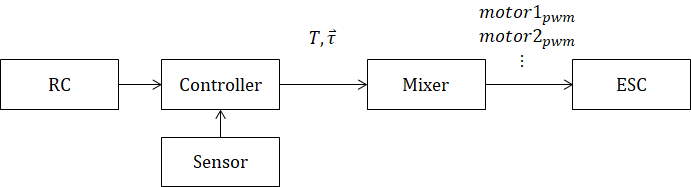
\includegraphics[width=0.95\linewidth]{figures/ch02/mixer_chain_docs.png}
    \caption[Vị trí khâu phân bổ lệnh động cơ trong chuỗi điều khiển multirotor.]{Vị trí khâu phân bổ lệnh động cơ trong chuỗi điều khiển multirotor~\cite{cookieroboticsMotorMixer}.}
    \label{fig:background-allocation-chain}
\end{figure}

\begin{samepage}
Theo quy ước cấu hình chữ X tại mục~\ref{subsec:background-configuration}, khoảng cách từ tâm thân đến mỗi trục rôto là $l$, với $a=l/\sqrt{2}$. Vị trí rôto 1 đến 4 lần lượt là trước trái, trước phải, sau phải và sau trái. Rôto 1 và 3 quay cùng chiều kim đồng hồ, rôto 2 và 4 quay ngược chiều kim đồng hồ khi nhìn từ trên xuống. Mômen phản lực truyền lên thân có chiều ngược với mômen dẫn động rôto. Do $z_B$ hướng xuống, rôto 1 và 3 tạo mômen yaw âm, rôto 2 và 4 tạo mômen yaw dương.
\par
\end{samepage}

Đặt $\mathbf f=[f_1,f_2,f_3,f_4]^\mathsf T$ và $\kappa=c_Q/c_T>0$. Từ tích có hướng giữa cánh tay đòn và lực $[0,0,-f_i]^\mathsf T$, quan hệ phân bổ được xác định:
\begin{equation}
    \underbrace{\begin{bmatrix}T\\\tau_x\\\tau_y\\\tau_z\end{bmatrix}}_{\mathbf U}
    =\underbrace{\begin{bmatrix}
        1&1&1&1\\
        a&-a&-a&a\\
        a&a&-a&-a\\
        -\kappa&\kappa&-\kappa&\kappa
    \end{bmatrix}}_{\mathbf A}
    \begin{bmatrix}f_1\\f_2\\f_3\\f_4\end{bmatrix}.
    \label{eq:background-allocation-matrix}
\end{equation}
Ở đây $f_i,T$ có đơn vị newton, $a,\kappa$ có đơn vị mét và $\tau_x,\tau_y,\tau_z$ có đơn vị $\mathrm{N\,m}$. Với $a,\kappa\ne0$, ma trận $\mathbf A$ khả nghịch; lực đẩy yêu cầu là:
\begin{equation}
    \begin{aligned}
        f_1^*&=\frac T4+\frac{\tau_x^*}{4a}+\frac{\tau_y^*}{4a}
            -\frac{\tau_z^*}{4\kappa},\\
        f_2^*&=\frac T4-\frac{\tau_x^*}{4a}+\frac{\tau_y^*}{4a}
            +\frac{\tau_z^*}{4\kappa},\\
        f_3^*&=\frac T4-\frac{\tau_x^*}{4a}-\frac{\tau_y^*}{4a}
            -\frac{\tau_z^*}{4\kappa},\\
        f_4^*&=\frac T4+\frac{\tau_x^*}{4a}-\frac{\tau_y^*}{4a}
            +\frac{\tau_z^*}{4\kappa}.
    \end{aligned}
    \label{eq:background-inverse-allocation}
\end{equation}
Các dấu trong \eqref{eq:background-inverse-allocation} phụ thuộc trực tiếp vào hệ trục, vị trí và chiều quay đã quy ước. Với bài toán roll và pitch, có thể đặt $\tau_z^*=0$ khi chưa triển khai vòng yaw. Khi đó, lực đẩy nền được phân phối đều, còn chênh lệch giữa các rôto tạo mômen hiệu chỉnh tư thế.

\subsection{Giới hạn lực đẩy và sai lệch sau phân bổ}

Độ lớn lực đẩy mỗi rôto thỏa mãn \mbox{$f_{\min}\le f_i\le f_{\max}$}. Giới hạn dưới có thể khác không khi động cơ duy trì tốc độ quay nền. Phép cắt biên trực tiếp cho lệnh khả thi:
\begin{equation}
    f_{i,a}=\operatorname{sat}_{[f_{\min},f_{\max}]}(f_i^*),
    \qquad \mathbf U_a=\mathbf A\mathbf f_a.
    \label{eq:background-allocation-saturation}
\end{equation}
Sau cắt biên, tổng lực đẩy và các mômen khả dụng nhìn chung khác giá trị yêu cầu. Sai lệch $\mathbf U^*-\mathbf U_a$ cho biết phần tác động không được thực hiện và cung cấp thông tin giới hạn cho bộ điều khiển. Nếu chỉ theo dõi từng lệnh riêng lẻ, ảnh hưởng của bão hòa đến khả năng ổn định tư thế có thể bị bỏ sót.

Một cách xử lý đơn giản là dịch cùng một lượng $\Delta f$ cho cả bốn lệnh trước khi cắt biên. Với các giới hạn giống nhau, điều kiện tồn tại lượng dịch khả thi là:
\begin{equation}
    f_{\min}-\min_i f_i^*\ \le\ \Delta f\ \le\
    f_{\max}-\max_i f_i^*.
    \label{eq:background-collective-shift}
\end{equation}
Do tổng hệ số của ba hàng mômen trong $\mathbf A$ bằng không, phép dịch chung bảo toàn các mômen yêu cầu và làm tổng lực đẩy đổi thành $T_a=T+4\Delta f$. Vì vậy, biện pháp này dành khoảng điều khiển cho tư thế bằng cách điều chỉnh lực đẩy nền; nó chỉ khả thi khi khoảng trong \eqref{eq:background-collective-shift} không rỗng. Khi độ chênh giữa các lệnh vượt $f_{\max}-f_{\min}$, cần giảm yêu cầu mômen hoặc dùng bài toán phân bổ có ràng buộc để thể hiện thứ tự ưu tiên. Phép cắt biên đơn thuần không bảo đảm đồng thời mọi yêu cầu điều khiển.

\subsection{Chuyển lực đẩy thành lệnh động cơ}

Với mô hình tĩnh $f_i=c_T\Omega_i^2$, tốc độ quay yêu cầu sau giới hạn là:
\begin{equation}
    \Omega_{i,d}=\sqrt{\frac{f_{i,a}}{c_T}},
    \qquad u_i=\mathcal H_i(\Omega_{i,d}),
    \label{eq:background-motor-command}
\end{equation}
trong đó $u_i$ là lệnh gửi đến bộ điều khiển tốc độ động cơ (ESC), còn $\mathcal H_i$ là quan hệ hiệu chuẩn trong miền làm việc. Quan hệ này phụ thuộc vào động cơ, cánh quạt, ESC và điều kiện nguồn. Lệnh PWM hoặc lệnh số chuẩn hóa biểu diễn mức yêu cầu của ESC; giá trị đó chỉ chuyển thành tốc độ quay thông qua đặc tính của cụm truyền động. Do đó, việc chuyển đổi được xây dựng từ mô hình hoặc dữ liệu hiệu chuẩn thay vì đồng nhất trực tiếp tốc độ rôto với giá trị lệnh.

Trong quá trình quá độ, tốc độ thực còn chịu quán tính của động cơ và cánh quạt. Có thể biểu diễn ảnh hưởng cơ bản bằng mô hình bậc nhất:
\begin{equation}
    T_m\dot\Omega_i+\Omega_i=\Omega_{i,d},
    \label{eq:background-motor-lag}
\end{equation}
với $T_m$ là hằng số thời gian tương đương. Mô hình này cho thấy lực đẩy không thay đổi tức thời theo lệnh, đồng thời giải thích vì sao tốc độ cập nhật cao của vi điều khiển không tự làm tăng tương ứng băng thông cơ cấu chấp hành. Các tham số hình học, giới hạn lực đẩy và quan hệ lệnh--tốc độ được xác định trong phần thiết kế để hoàn thiện chuỗi từ mômen yêu cầu đến tác động lên quadrotor.
